\documentclass[letter,twocolumn]{article}
\usepackage{tutorial}
\usepackage[OT1]{fontenc}

% ------------------------------------------------------------------------
\usepackage{graphicx}
\usepackage{subfigure}
\usepackage{epsfig}
\usepackage{psfrag}
% used to write c++ code/algorithms
\usepackage{listings}
\usepackage{fancyvrb}

%\psdraft

\twocolumn


% hyperref stuff
\usepackage{hyperref}
\hypersetup{
  pdftitle={A Tutorial on CGAL Polyhedron for Subdivision Algorithms},
  pdfauthor={INRIA Geometrica},
  pdfsubject={A tutorial for CGAL},
  pdfkeywords={},
  pdfpagemode=UseThumbs,
  baseurl={http://www.cgal.org},
  colorlinks=true,
  linkcolor=black,
  anchorcolor=black,
  citecolor=black,
  filecolor=black,
  menucolor=black,
  pagecolor=black,
  urlcolor=blue,
  bookmarksopen=false,}
% end hyperref stuff

\lstset{language=C++, basicstyle=\scriptsize}

\graphicspath{{figs/}}
\def\figurename{Figure}
\def\tablename{Tableau}
\newcommand{\italic}[1]{\emph{#1}} 

% ------------------------------------------------------------------------
\newcommand\IL{{\itshape left}}
\newcommand\IR{{\itshape right}}
\newcommand\IM{{\itshape middle}}
\newcommand\IT{{\itshape top}}
\newcommand\IB{{\itshape bottom}}

% ------------------------------------------------------------------------
\newcommand{\CodeFmt}[1]{{\small\texttt{#1}}}

\def\kernel{\CodeFmt{Kernel}}

\def\cgalpoly{\CodeFmt{CGAL::Polyhedron\_3}}
\def\poly{\CodeFmt{Polyhedron\_3}}
\def\polytrait{\CodeFmt{PolyhedronTraits\_3}}
\def\polyitem{\CodeFmt{PolyhedronItems\_3}}
\def\polybuilder{\CodeFmt{Polyhedron\_incremental\_builder\_3}}

\def\cgalhds{\CodeFmt{CGAL::HalfedgeDS}}
\def\hds{\CodeFmt{HalfedgeDS}}
\def\hdsitem{\CodeFmt{PolyhedronItems}}

% L.K. -------------------------------------------------------------------
\newcommand{\CC}{C\raise.08ex\hbox{\texttt{++}}}
\newcommand{\openmesh}{\textsc{OpenMesh}}
\newcommand{\opensg}{\textsc{OpenSG}}
\newcommand{\cgal}{\textsc{Cgal}}
\newcommand{\stl}{\textsc{Stl}}


% =========================================================================
\begin{document}

% TITLE
% ------------------------------------------------------------------------
\date{}
\title{{\LARGE {\sffamily\bfseries A Tutorial on CGAL Polyhedron \\
                                   for Subdivision Algorithms}}}


\author{\small
\sffamily Le-Jeng Shiue\footnote{SurfLab, University of Florida}
\and \small
\sffamily Pierre Alliez\footnote{GEOMETRICA, INRIA Sophia-Antipolis}
\and \small
\sffamily Radu Ursu\footnote{Geometry Factory, Sophia-Antipolis}
\and \small
\sffamily Lutz Kettner\footnote{MPII, Saarbr\"ucken}}
\maketitle

\thispagestyle{empty}

% ABSTRACT
% ------------------------------------------------------------------------
\abstract{
We will present a tutorial on the CGAL polyhedron data structure
assuming familiarity with the C++ template mechanism and the key
concepts of the generic programming. The tutorial is organized around
a mesh subdivision application.  It starts with a polyhedron viewer
for a customized polyhedron.  The polyhedron viewer demonstrates the
basic functionalities of the \cgalpoly\ and some extended
functionalities such as file I/O, mesh superimposition, and trackball
manipulation.  The tutorial also shows how to implement subdivision
algorithms in three different approaches. These approaches are
proposed with increasing level of sophistication and abstraction. The
simplest approach uses the atomic operators of the combinatorial
modifications to implement $\sqrt{3}$ subdivision scheme.  A second
approach overloads the modifier, with the help of the incremental
builder, to implement quad-triangle subdivision. The third approach
abstracts the geometry operations from the refinements.  It
specializes a subdivision with template geometry rules. Catmull-Clark,
Loop and Doo-Sabin subdivisions are illustrated based on this third
approach.  }

%%\vskip 3mm

\begin{center} 
  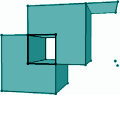
\includegraphics[width=\linewidth]{figs/teaser}\\ {\scriptsize Demo
  application running on Windows. A coarse polygon mesh is subdivided
  using the quad-triangle subdivision scheme.}
\end{center}

\subsection*{Generic Mesh Data Structure}

Polyhedron data structures based on the concept of halfedges have been
very successful for the design of general algorithms on meshes.
Although making a preliminary version of a halfedge-based mesh data
structure (HDS) is as a fairly simple task and is often proposed as a
programming exercise, there now exists a general purpose HDS available
which is worth considering relying on. With the successful use of
generic programming in C++, a set of reusable library components for
graphics modeling and geometry processing are demanded by researchers
and developers. \italic{Extensible algorithm} models based on a
\italic{robust, efficient and customizable polyhedron data structure}
will certainly speed up the research as well as the development cycle,
and benefit the community of geometric computing and geometry
processing.

Most mesh algorithms employ a customized halfedge data structures and
most of the customizations are specialized by customizing the
primitive data, which are the vertex positions, the facet normals or
other data used for algorithmic purposes. \cgalpoly\ encapsulates a
generic design of the halfedge data structure allowing users customize
the \poly\ with the template parameters of the geometry
primitives. There are several advantages employing the \poly\ as the
core data structure of a mesh processing application: \\

\indent $\bullet$ The \poly\ is a \italic{generic} data structure.\\
\indent $\bullet$ The \poly\ is a \italic{robust} and \italic{optimized} 
                  data structure.\\
\indent $\bullet$ A complete set of geometric entities and predicates
                  is provided within CGAL.\\
\indent $\bullet$ CGAL is closely following the programming 
                  style of the C++ STL.

% todo: explain why polyhedron_3 is a generic data structure

\subsection*{Demo Application}

We have designed and implemented an application based on the
\cgalpoly. This program provides a polyhedron viewer of
following functionalities:\\
\indent $\bullet$ File I/O,\\
\indent $\bullet$ polyhedron rendering,\\ 
\indent $\bullet$ and trackball manipulation.\\
In addition to these built-in functions, the viewer is accompanied
with a set of subdivision algorithms that generate smooth polyhedron
surfaces from a coarse polyhedron. \italic{The tutorial instructs the
readers through the design and the implementation of the polyhedron
viewer and the subdivisions}. The first part of the tutorial
highlights the design and implementation issues related to the \poly\
used in the viewer. The second part of the tutorial explains how to
implement the connectivity and geometry operations of the subdivision
algorithms. The source codes are going to be published with the
releasing of the tutorial.

\subsection*{Tutorial Outlines}
\subsubsection*{Polyhedron Viewer}

The tutorial starts with demonstrating how to implement a simple
viewer based on the default configuration of the \cgalpoly . This
simple viewer demonstrates some basic functionalities of the
\cgalpoly\ such as \italic{modifier} and \italic{incremental builder} 
for initialization and the mesh traversal, i.e. the \italic{iterators}
and the \italic{circulators}, for rendering or mesh exporting. Based
on this simple viewer, we then show the readers how to
\italic{customize the \poly} to support certain functionalities. 
An enriched polyhedron is proposed with the primitives specialized
with algorithmic flags. This enriched polyhedron is used as the core
data structure of our application.  We then show how to interact with
a customized \poly.  The extended primitives are employed to support
the superimposition of the input mesh on the subdivided surfaces. A
trackball function of the enriched polyhedron is also demonstrated in
the tutorial.

\subsubsection*{Subdivision Algorithms}

The second part of the tutorial focuses on the design and the
implementation of the subdivision algorithms.  In addition to the
importance in surface modeling, we choose subdivision algorithms to
demonstrate both the \italic{topology operation} (refinement) and the
\italic{geometry operations} (smoothing). The topology and the geometry
operations are the two basic operations required by most geometry
algorithms. Our implementations of the subdivisions are designed to be
a separated library that accepts any generic \poly\ as the input
polyhedron (not just the enriched polyhedron we used in the polyhedron
viewer). The key to implement a subdivision algorithm is to support
the refinement, i.e.\ the connectivity modifications.  Two approaches
are first introduced to support the refinement: the \italic{atomic
operators of the combinatorial modifications} (operator scheme) and
the \italic{modifier mechanism} (modifier scheme).  The operator
scheme reconfigures the connectivity with a combination of several
combinatorial operators. The $\sqrt{3}$ subdivision~\cite{sqrt3} is
used to demonstrate this scheme. Though simple and efficient in some
refinements, e.g.\ $\sqrt{3}$ subdivision, the correct combination of
the operators is hard to find for some refinements, e.g.\ Doo-Sabin
subdivision~\cite{ds}. The modifier scheme solves the problem by
letting the programmers create their own combinatorial operators using
the polyhedron incremental builder.  The Quad-Triangle
subdivision~\cite{qts,l-pg-03} is used to demonstrate this scheme.

\subsubsection*{Generic Subdivisions}

Subdivisions can be represented as a combination of a refinement and a
set of smoothing rules. Based on this observation, our third approach
generalizes the subdivision by abstracting the smoothing rules from
the refinement. The refinement is designed as a \italic{host function}
that accepts a \italic{policy class} supporting the smoothing rules. A
subdivision function is then a legal combination of the refinement and
the smoothing rules.  For example, the Catmull-Clark
subdivision~\cite{cc} can be declared as:
\begin{lstlisting}
void CatmullClark_subdivision(Polyhedron& p) {    
  quadralize_polyhedron
   <CatmullClark_rule<Polyhedron>>(p);  
}
\end{lstlisting}

The \lstinline!quadralize_polyhedron<>! represents the refinement
(host function) and the \lstinline!CatmullClark_rule<>! supports the
geometry rules (policy).  This approach offers a convenient way to
specialize a subdivision with the \italic{template smoothing rules}.
Catmull-Clark~\cite{cc}, Loop~\cite{loop} and Doo-Sabin~\cite{ds}
subdivisions are illustrated based on this approach.

\subsection*{Intended Audience}

The intended audience of the tutorial are researchers, developers or
students developing algorithms around meshes. Experience in advanced
C++ design (i.e.\ generic programming using templates) and knowledge
of the halfedge data structure and subdivisions are prerequisites.

% references
{\footnotesize
\bibliographystyle{alpha}
\bibliography{abstract}
}

\end{document}
